% \subsection{The Implementation Evaluation Results }
% \label{sec:adapt-impleval}

We implemented $\THESYSTEM$ as a tool that takes a labeled command as input 
and outputs two upper bounds on the program adaptivity and the number of query requests respectively.
This implementation consists of an 
abstract control flow graph generation,
edge estimation (as presented in Section~\ref{sec:alg_edgegen}), and weight estimation (as presented in Section~\ref{sec:alg_weightgen}) in Ocaml, 
and the adaptivity computation algorithm shown in Section~\ref{sec:alg_adaptcompute} in Python.
The OCaml program takes the labeled command as input and outputs the program-based dependency graph and
the abstract transition graph,
feeds into the python program and the python program provides the adaptivity upper bound and the query number as the final output.

We evaluated this implementation on $23$ example programs with the evaluation results shown in Table~\ref{tb:adapt-imp}.
{\footnotesize
\begin {table}[H]
\vspace{-0.4cm}
    \caption{Accuracy and Performance Evaluation of {\THESYSTEM} implementation}
    \vspace{-0.5cm}
        \label{tb:adapt-imp}
        \begin{center}
        \centering
{\tiny
        \begin{tabular}{| >{\tiny}r | c | c | c | c | c | c | c | c | c | c | c }
         \hline \hline
        \multirow{2}{*}{Program $c$} & 
        \multirow{2}{*}{\emph{adaptivity}}
         & \multicolumn{2}{c|}{$\THESYSTEM$}
         & {L.O.C}
         & \multicolumn{3}{c|}{running time (second)} \\ 
         \cline{3-8}
         & & {$\progA$ } & {$\query$\# } &  & graph & weight & $\pathsearch$ \\ 
         \cline{6-8}
        %  & & & &  & $\THESYSTEM$-I & $\THESYSTEM$-II & $\THESYSTEM$-III  \\
         \hline \hline
         $  \kw{twoRounds(k)}$ & $2$ &  $2$ & $k+1 $  & 8 & 0.0005 & 0.0017 & 0.0003 \\
         $  \kw{mR(k)}$ & $k$ &  $k$ & $k$  &  10 & 0.0012 & 0.0017  & 0.0002 \\
         $  \kw{lRGD(k, r)}$ & $k$ & $k  $ & $ 2k $  &  10 & 0.0015 & 0.0072  & 0.0002  \\
         $  \kw{mROdd(k)}$ & $1 + k$ &  $2+\max(1,2k)  $ & $1 + 3 k  $  &  10 & 0.0015 & 0.0061  & 0.0002 \\
         $  \kw{mRSingle(k)}$    & $2$ &  $1+ \max(1, k) $ & $1 + k $  &  9 & 0.0011 & 0.0075  & 0.0002 \\
        %  $  \kw{seq()}$ & $4$ & $4$ & $4$ & 4 & 0.0016 & 0.0002 & 0.0001 \\ 
         $  \kw{seqRV()}$ & $4$ & $4$ &  $4$ & 4 & 0.0011 & 0.0003 & 0.0001 \\  
         $  \kw{ifVD()}$ & $2$ & $2$ &  $3$ & 5 & 0.0010 & 0.0005  & 0.0001 \\
         $  \kw{ifCD()}$ & $3$ & $3 $ &   $3$  & 5 & 0.0005 & 0.0003   & 0.0001 \\
         $  \kw{loop(k)}$ & $1+k/2$ &   $1 +\max(1, k/2)  $  &  $1+k/2  $ & 7 & 0.0021 & 0.0015 &  0.0001 \\
         $  \kw{loopRV(k)}$ & $1 + 2k$ &  $1 + 2k$ & $2 + 3 k$  &  9 & 0.0016 & 0.0056 & 0.0001  \\
         $  {\kw{loopVCD(k)}} $ & ${1 + 2Q_m}$ &  ${Q_m+\max(1,2Q_m)}$  & $2+2Q_m$   &  6 & 0.0016 & 0.0007 & 0.0001 \\
         $ {\kw{loopMPVCD(k)}}$ & $2+Q_m$ &  $2 + Q_m$  & $2+2Q_m$   &   9 & 0.0017 & 0.0043  & 0.0001 \\
         $  \kw{loop2VD(k)}$ & $2 + k^2$ &   $3 + k^2$ & $1 + k + k^2 $   &  10 & 0.0018 & 0.0126  & 0.0001  \\
         $  \kw{loop2RV(k)}$ & $1 + k +  k^2$ &  
         $ 2 + k +  k^2 $ 
         &  $2 + k + k^2$   &  10 & 0.0017 & 0.0186  & 0.0001  \\
         $  \kw{loop2MV(k)}$ & $1 + 2k $ & $1 + \max(1,2k) $ &  $1 + k + k^2 $  & 10 & 0.0016 & 0.0071  & 0.0001 \\
         $ \kw{loop2MPRV(k)}$ & $1 + k + k^2$ &  $3 + k + k^2  $ &  $2 + 2k + k^2  $  &  10 & 0.019 & 0.0999  & 0.0002 \\
         {$ \kw{loopM(k)}$} & $1 + k$ &  $ 2 + \max(1,2k) $ & $1 + 3k  $  &  9 & 0.0017 & 0.0062  & 0.0001  \\
         {$ \kw{loopM2(k)}$} & $1 + k$ &  $ 2 + k $ & $1 + 3k  $  &  9 & 0.0017 & 0.0062  & 0.0001  \\
         {$\kw{loop2R(k)}$} & $1 + 3k$ &  $1 + 3k $ &  $1 + 3k  + k^2$  &  11 & 0.019 & 0.2669  & 0.0007 \\
         $  \kw{mR(k, N)}$ & $k$ & $ k   $ & $k $   &  27 & 0.0026 & 85.9017  & 0.0004 \\
         $  \kw{mRCom(k)}$ & $2k$ & $  2k $ & $ 2k $   &  46 & 0.0036 & 5104  &  0.0013\\
         $  \kw{seqCom(k)}$ & $12$ & $12  $  & $326 $  &  502 & 0.0426  & 1.2743  & 0.0223 \\
         $  \kw{tRCom(k)}$ & $2$ &  $ * $ & $*  $  &  42 & 0.0026 & $*$  & $*$\\
         $  \kw{{jumbo(k)}}$ & $ \max(20, 8+k^2)$ &  $ * $   &   $* $  &  71 & 0.0035 & $*$ &  $*$ \\
        %  $  \kw{jumbo(k)}$ & $ \max(20, 10+k+k^2 )$ &   $* | \max(20, 12 + k+ k^2)$  &  $* |286+26k+10k^2$   &  502 & 0.0691 & * | 0.0009 & 0.018 \\
         $  {\kw{big(k)}} $ & $22+k+k*k$ &  $* $ &  $* $  &  214 & 0.0175 & $*$ & $*$ \\
         \hline \hline
        \end{tabular}
}
\end{center}
\end{table}
}




In this table,
the first column is the name of each program.
For each program $c$, the second column is its intuitive adaptivity rounds,
and the third column is the output of the $\THESYSTEM$ implementation, which consists of two expressions.
The first one is the upper bound for adaptivity and the second one is the 
upper bound for the total number of query requests in the program. And the last column is the performance evaluation w.r.t. the program size.

The last column is the performance evaluation.
The time contains three parts. The first part is the running time of the Ocaml code, which parses the program and generates the $\progG(c)$.
The second and third parts are the running times of the reachability bound analysis algorithm
and the adaptivity computation algorithm, $\pathsearch(c)$.

The first six programs are adapted from real-world data analysis algorithms.
The first two programs $\kw{twoRounds(k)}$, $ \kw{multiRounds(k)}$ are the same as Figure~\ref{fig:overview-example}(a) and Figure~\ref{fig:multipleRounds}(a).
$\THESYSTEM$ computes tight adaptivity bound for the first three examples.
For the fourth program $\kw{multiRoundsO(k)}$, $\THESYSTEM$ outputs an over-approximated upper bound $1 + 2*k$ 
% for the $A(c)$, which is consistent with our expectation 
as discussed in Example~\ref{ex:multiRoundsO}. 
The fifth program is the evaluation results for the example in Example~\ref{ex:multiRoundsS}, where $\THESYSTEM$ outputs the tightly bound for $A(c)$ but $A(c)$ is a loose definition of the program's actual adaptivity rounds.
%

The next eleven programs from Table~\ref{tb:adapt-imp} rows 7 to 18 are handcrafted programs based on the code pieces extracted from the C library. They all have small sizes but complex structures in order to test the programs under different situations including
data, control dependency,
the multiple paths nested loop with related counters, etc.
The names of these programs obey the convention that,
$\kw{if}$ means there is if control in the program;
$\kw{loop}$ means there is while loop and $\kw{loop2}$ represents two levels nested loop in the program;
$\kw{C}$ denotes Control;
$\kw{D}$ for Dependency; $\kw{V}$ for Variable;
$\kw{M}$ for Multiple; $\kw{P}$ for Path and $\kw{R}$ for Related.


The algorithm computes the tight bound for examples from line six, $\kw{ifCD()}$ to line fourteen, $\kw{loop2MPRV(k)}$
and over-approximate the \emph{adaptivity} for the $15^{th}$ and $16^{th}$ examples in the table due to path-insensitivity.

The last six programs are synthesized programs composed of the previous programs in order to test the performance limitation when the input program is large. 
From the evaluation results, the performance bottleneck is the reachability bound analysis algorithm.


By implementing the bound analysis algorithm in Section~\ref{sec:alg_weightgen} (adapted from \cite{SinnZV17}), we are unable to evaluate the $\kw{Jumbo}$ in a reasonable time period.
Alternatively, we implement another light reachability bound analysis algorithm and compute the \emph{adaptivity} for
$\kw{jumboS}, \kw{jumbo}$ and $\kw{big}$ effectively.
We also show our alternative implement evaluation result in Table~\ref{tb:adapt-imp-alternatives}.
The alternative implementation computes the tight bound for all the examples from line:1 to line:14
and over-approximate the \emph{adaptivity} for $15^{th}$ and $16^{th}$ due to path-insensitivity similar to the
$\THESYSTEM$.
For the $17^{th}$ example ($\kw{loop2RC}$), {\THESYSTEM} gives a tight bound while the alternative implementation gives a loose bound, so we keep both implementations.

Overall, {\THESYSTEM} gives the accurate estimated
adaptivity upper bound and our adaptivity formalization also gives precise adaptivity definition w.r.t. the intuitive \emph{adaptivity rounds}.
% and analysis framework $\THESYSTEM$.
{\footnotesize
\begin {table}[H]
\vspace{-0.2cm}
    \caption{Accuracy Evaluation of {\THESYSTEM}  Alternative Implementations}
    \vspace{-0.2cm}
        \label{tb:adapt-imp-alternatives}
        \begin{center}
        \centering
{\tiny
        \begin{tabular}{ | >{\tiny}r | c | c | c | c | c | c | c | c | c | c | c |}
        \hline \hline
        \multirow{2}{*}{Program $c$}
         & \multicolumn{2}{c|}{$\THESYSTEM$-I}
         & \multicolumn{2}{c|}{$\THESYSTEM$-II}
         & \multicolumn{2}{c|}{$\THESYSTEM$-III}
         & \multicolumn{3}{c|}{running time (second)} \\ 
         \cline{2-10}
         & {$\progA$ } & {$\query$\# } & {$\progA$ } & {$\query$\# } & {$\progA$ } & {$\query$\# } & $\THESYSTEM$-I & $\THESYSTEM$-II & $\THESYSTEM$-III \\ 
         \cline{5-10}
        %  & & & &  & $\THESYSTEM$-I & $\THESYSTEM$-II & $\THESYSTEM$-III  \\
         \hline \hline
         $  \kw{twoRound(k)}$ &  $2$    & $k+1 $  & & & $2$ & $k + 1$ & 0.0010 &  & 0.00656 \\
         $  \kw{mR(k)}$ &   $\max(1,k)$ & $k$  &  & & & & 0.0016 & & \\
         $  \kw{lRGD(k, r)}$ & $\max(1,k) $ & $ 2k $  &  & & & & 0.0019 & &  \\
         $  \kw{mROdd(k)}$  &  $2+\max(1,2k)  $ & $1 + 3 k  $  &  & & & & 0.0019 & &\\
         $  \kw{mRSingle(k)}$    & $1+ \max(1, k) $ & $1 + k$  &  & & & & 0.0015 & & \\
         $  \kw{ifCD()}$   & $4$ &   $4$  & & & & & 0.0007 & & \\
         $  \kw{loop(k)}$ &    $1 + \max(1, \frac{k}{2}) $  &  $1+\frac{k}{2} $ & & & & & 0.0023 &  & \\
         $  \kw{loopRV(k)}$   &  $ 1 + \max(1,2k)$ & $2 + 3 k$  &  & & & & 0.0019 & & \\
         $  {\kw{loopVCD(k)}} $  &  ${Q_m+\max(1,2Q_m)}$  & $2+2Q_m$   &  & & & & 0.0019 & & \\
         $ {\kw{loopMPVCD(k)}}$  &  $2 + Q_m$  & $2+2Q_m$   &   & & & & 0.0020 & & \\
         $  \kw{loop2VD(k)}$  &   $3 + k^2$ & $1 + k + k^2$   &  & & & & 0.0021 & & \\
         $  \kw{loop2RV(k)}$  &  $ 2 + k +  k^2 $    &  $2 + k + k^2$   &  & & & & 0.0021 & & \\
         $  \kw{loop2MV(k)}$  & $1 + \max(1,2k) $ &  $1 + k + k^2 $  & & & & & 0.0019 & & \\
         $ \kw{loop2MPRV(k)}$  &  $3 + k + k^2  $ &  $2 + 2k + k^2  $  &  & & & & 0.0194 & & \\
         {$ \kw{loopM(k)}$}  &  $ 2 + \max(1,2k) $ & $1 + 3k  $  &  & & & & 0.0021 & & \\
         {$ \kw{loopM2(k)}$}  &  $ 2 + k $ & $1 + 3k  $  &  & & & & 0.0021 & & \\
         {$\kw{loop2RC(k)}$}&  $2 + 3k + k^2$ &  $1 + k + k^2$  &  & & & & 0.0199 & & \\
         $  \kw{mR(k, N)}$ & $ k   $ & $k $   &  & & & & 0.0033 & & \\
         $  \kw{mRC(k)}$  & $  2k $ & $ 2k $   &  & & & & 0.0052 & & \\
         $  \kw{seqC(k)}$ & $12  $  & $326 $  &  & & & & 0.0652 & & \\
         $  \kw{tRC(k)}$ &  $ 2$ & $ 1 + 5k + 2 k^2 $  &  & & & & 0.0034 &  & \\
         $  \kw{{jumbo(k)}}$ & $  \max(20, 6+k+k^2)$   &   $ {44+k+k^2} $  &  & & & & 0.0123 &  & \\
         $  {\kw{big(k)}} $ &   $28 + k + k^2$ &  $121+11k+4k^2 $  &  & & & & 0.0181 & & \\
        \hline \hline 
        \end{tabular}
}
\end{center}
\end{table}
}





We evaluate our framework also on the real-world programs from
three benchmark sets, including thensorflow, sklearn and pytorch and research paper~\cite{Jamieson2015TheAO}.
{\footnotesize
\begin {table}[t]
        \vspace{-0.5cm}
        \caption{Evaluation of Data Analyses Generalization Error Using {\THESYSTEM}}
    \vspace{-0.4cm}
        \label{tb:adapt-generalization}
        \begin{center}
        \centering
{
        \begin{tabular}{|| >{\tiny}l || c | c |c || c || l | c | r ||  }
                \hhline{t|:======== :t:|}
        \multirow{2}{*}{Program $c$}
         & \multicolumn{2}{c}{$\THESYSTEM$}
         & &{rmse}
         & \multicolumn{3}{c||}{rmse with mechanisms} \\ 
        %  \cline{2-3} 
         \hhline{||~---||~---||}
        %  \cline{5-7}
         & {$\progA$ } & {$\query$\# } & real value &   & Data Split & Gaussian & Threshold  \\ 
         \hline \hline
        %  \hhline{|| = || = | = || = || = | = | = || }
        % \hhline{|:t ======== t:|}
        $  \kw{ twoRounds }$ & $ 2 $ & $  k + 1 $ & $ k = 1000$ & $0.050$   & {\textbf{0.028}} & {$0.031$} & $0.040$  \\
        \hhline{||-||---||-||---||}
        $  \kw{ twoRounds }$ & $ 2 $ & $  k + 1 $ & $ k =  1$ & $0.0006$   & {{$0.0015$}} & \textbf{0.0004} & {$0.001$}  \\
        \hhline{||-||---||-||---||}
         $  \kw{ mR}$ & $k$ & $k$ & $ k =  1000$  & $0.066$   & $0.050$ & {\textbf{0.036}} & $0.064$  \\
         \hhline{||-||---||-||---||}
         $  \kw{ mR}$ & $k$ & $k$ & $ k =  10$  & $0.16$   & $0.1545$  & $0.108674 $ & \textbf{0.1035}  \\
         \hhline{||-||---||-||---||}
         $  \kw{ mROdd }$ & $ k $   & $  2 \times k $& $ k =  1000$ & $0.211$   & $0.220$ & {\textbf{0.059}} & $0.171$  \\
         \hhline{||-||---||-||---||}
         $  \kw{ mROdd }$ & $ k $   & $  2 \times k $& $ k =  5$ & $0.9375$   & $0.999$ & $0.7427$ & {\textbf{0.4016}}  \\
         \hhline{||-||---||-||---||}
         $  \kw{ mRSingle }$ & $ k $ & $  k $ & $ k =  1000$  & $ 0.761$   & $ 0.758$ & {\textbf{0.509}} & $ 0.593$  \\
         \hhline{||-||---||-||---||}
         $  \kw{ mRSingle }$ & $ k $ & $  k $ & $ k =  10$  & $0.8074$   & $0.3600$ & $ 0.7506$ & {\textbf{0.4036}}  \\
         \hhline{||-||---||-||---||}
         $  \kw{ lRGD }$ & $ k $ & $  2\times k $ & $ k =  1000$  & $0.216$   & $0.209$ & \textbf{0.014} & $0.210$  \\
         \hhline{||-||---||-||---||}
         $  \kw{ lRGD }$ & $ k $ & $  2\times k $ & $k =  10$  & $0.12$   & $0.116$ & $ 0.1 $ & \textbf{0.06}  \\
         \hhline{||-||---||-||---||}
         $  \kw{ 3DimLRGD }$ & $ k $ & $  3\times k $ & $ k =  1000$  & $0.1966$   & $0.1901$ & \textbf{0.1751} & $0.1810$  \\
         \hhline{||-||---||-||---||}
         $  \kw{ 3DimLRGD }$ & $ k $ & $  3\times k $ & $ k =  10$  & $0.1159$   & $0.1$ & $0.1079$ & \textbf{0.092}  \\
         \hhline{||-||---||-||---||}
         $  \kw{ 4DimLRGD }$ & $ k $ & $  4\times k $ & $ k =  1000$  & $0.1112$   & $0.1032$ & \textbf{0.0961} & $0.1000$  \\
         \hhline{||-||---||-||---||}
         $  \kw{ 4DimLRGD }$ & $ k $ & $  4\times k $ & $ k =  10$  & $0.6$   & $0.1080$ & $0.3 $ & \textbf{0.1399}  \\
         \hhline{||-||---||-||---||}
         $  \kw{ 3DegreeLRGD }$ & $ k $ & $  3\times k $ & $ k =  1000$  & $0.1096$   & $0.1056$ & \textbf{0.0098} & $0.1004$  \\
         \hhline{||-||---||-||---||}
         $  \kw{ 4DegreeLRGD }$ & $ k $ & $  4\times k $ & $ k =  1000$  & $0.1084$   & $0.1058$ & \textbf{0.1052} & $0.1055$  \\
         \hhline{||-||---||-||---||}
         $\kw{repeatedQuery}$~\cite{Jamieson2015TheAO} & $ m \times 2^m $ & $  m \times 2^m $ & $ k =  1000$  & $239.0$   & $21.5$ & {\textbf{18.557}} & $141.974$  \\
         \hhline{||-||---||-||---||}
         $\kw{nDimPairwise}$~\cite{Jamieson2015TheAO} & $ m $ & $  m \times n  $ & $ n,m =  1000$  & $0.0999$   & $0.0999$ & $0.0970$ & \textbf{0.0999}  \\
         \hhline{||-||---||-||---||}
         $\kw{bestArm}$~\cite{Jamieson2015TheAO} & $ n $ & $  m \times n $ & $ n,m =  1000$  & $ 2.0452$   & $ 1.3955$ & {{$3.4147$}} & \textbf{1.2871}  \\
         \hhline{||-||---||-||---||}
         $\kw{lilUCB}$~\cite{Jamieson2015TheAO} & $ n $ & $ m \times n $ & $ n,m =  1000$ & $3.0174$   & $ 3.137$ & {$3.5245$} & \textbf{2.3865}  \\
         \hhline{||-||---||-||---||}
         $\kw{decisionTree}$ & $k$ &  $k$ & $ n,m =  1000$ & $ 1.465$  & $ 1.283$ & \textbf{1.379 } & {$1.414$}  \\
         \hhline{||-||---||-||---||}
         $\kw{logisticRegression}$ & $k$ &  $k$ & $ n,m =  1000$ & $ 0.152$  &  $ 0.001$ & {\textbf{0.001}} & {$0.002$}   \\
        %  $  \kw{naiveGaussianB}$ & $100$ & $k  $ &  $ -  $  &  $-$ & $-$ & $-$ \\
        \hhline{||-||---||-||---||}
        $\kw{decisionTreeOVR}$ & $k \times m$ &  $ k \times m $ & $ k,m =  1000$ &  $0.055$ & $0.053$  &  {\textbf{0.007}} & $0.036$  \\
        \hhline{||-||---||-||---||}
        $\kw{logisticRegressionOVR}$  & $k \times m$ &  $ k \times m $ & $ k,m =  1000$ &  $ 1.000  $  &  $ 1.000 $ & {\textbf{ 0.999}} & $ 1.002 $ \\
        %  $  \kw{naiveGaussianOVR}$ & $n\times m$ & $ $ &  $ -  $  &  $-$ & $-$ & $-$ \\
        %  $  \kw{oneDenseLayer}$ & $ k \times m  $  & $ k \times m $   &  $ 1.567029  $  &  {$ 1.5590129 $} & $1.6002096$ & {\textbf{ 1.5671146 $}  \\
        %  {$ \kw{twoDenseLayer}$} & $ k \times m  $  & $ k \times m $ &  $ 300.27667 $  &  $ 292.82684 $ & $ 260.21957 $ & {\textbf{ 188.14603 $}  \\
        %  $  \kw{RNN}$           & $ k \times m  $  & $ k \times m $ &  $ 136.82417 $  &  $ 115.84269 $ & $ 122.5177 $ & {\textbf{ 126.23619 $}  \\
        % %  $  \kw{statefulRNN}$   & $ n $   &   $ n $ &  $ -  $  &  $-$ & $-$ & $-$ \\
        %  $  \kw{LSTM}$          & $ k \times m $   &  $ k \times m $  &  $ 3.2286646  $  &  $ 3.212278 $ & $3.0805347$ & {\textbf{{2.7898219}$}  \\
        %  $  \kw{twoLayerLSTM}$  & $ k \times m $ &  $ k \times m $  &  $ 3.465096  $  &  $3.2795377$ & {${2.2387855}$} & {\textbf{2.1549027$}  \\
        % %  {$ \kw{transferLearning}$} & $n$ &  $ n $ &  $ -  $  &  $-$ & $-$ & $-$ \\
        % %  {$\kw{imageRetrain}$} & $n$ &  $ n $ &   $ -  $  &  $-$ & $-$ & $-$ \\
        %  $ \kw{CNN}$ & $ k \times m $ &  $  k \times m $ &  $54.197838$  &  $44.91098$ & $48.472355$ & {\textbf{45.13651$}  \\
        %  $ \kw{CNNwithLSTM}$ & $ k \times m $ &  $ k \times m $ &  $ 12.198408  $  &  $  8.806086$ & $ 10.579981 $ & {\textbf{ 6.6821547 $} \\
        \hhline{|:t======== t:|}
\end{tabular}
}
\end{center}
\vspace{-0.5cm}
\end{table}
}


% {\footnotesize
% \begin {table}[t]
%         \vspace{-0.5cm}
%         \caption{Evaluation of Data Analyses Generalization Error Using {\THESYSTEM}}
%     \vspace{-0.4cm}
%         \label{tb:adapt-generalization}
%         \begin{center}
%         \centering
% {
%         \begin{tabular}{|| >{\tiny}l || c | c |c || c || l | c | r ||  }
%                 \hhline{t|:======== :t:|}
%         \multirow{2}{*}{Program $c$}
%          & \multicolumn{2}{c}{$\THESYSTEM$}
%          & &{rmse}
%          & \multicolumn{3}{c||}{rmse with mechanisms} \\ 
%         %  \cline{2-3} 
%          \hhline{||~---||~---||}
%         %  \cline{5-7}
%          & {$\progA$ } & {$\query$\# } & real value &   & Data Split & Gaussian & Threshold  \\ 
%          \hline \hline
%         %  \hhline{|| = || = | = || = || = | = | = || }
%         % \hhline{|:t ======== t:|}
%         $  \kw{ twoRounds }$ & $ 2 $ & $  k + 1 $ & $ k = 1000$ & $0.050$   & {\textbf{0.028}} & {$0.031$} & $0.040$  \\
%         \hhline{||-||---||-||---||}
%         $  \kw{ twoRounds }$ & $ 2 $ & $  k + 1 $ & $ k =  1$ & $0.0006$   & {{$0.0015$}} & \textbf{0.0004} & {$0.001$}  \\
%         \hhline{||-||---||-||---||}
%          $  \kw{ mR}$ & $k$ & $k$ & $ k =  10$  & $0.066$   & $0.050$ & {\textbf{0.036}} & $0.064$  \\
%          \hhline{||-||---||-||---||}
%          $  \kw{ mROdd }$ & $ k $   & $  2 \times k $& $ k =  1000$ & $0.211$   & $0.220$ & {\textbf{0.059}} & $0.171$  \\
%          \hhline{||-||---||-||---||}
%          $  \kw{ mRSingle }$ & $ k $ & $  k $ & $ k =  1000$  & $ 0.761$   & $ 0.758$ & {\textbf{0.509}} & $ 0.593$  \\
%          \hhline{||-||---||-||---||}
%          $  \kw{ lRGD }$ & $ k $ & $  2\times k $ & $ k =  1000$  & $0.216$   & $0.209$ & \textbf{0.014} & $0.210$  \\
%          \hhline{||-||---||-||---||}
%          $  \kw{ 3DimLRGD }$ & $ k $ & $  3\times k $ & $ k =  1000$  & $0.1966$   & $0.1901$ & \textbf{0.1751} & $0.1810$  \\
%          \hhline{||-||---||-||---||}
%          $  \kw{ 4DimLRGD }$ & $ k $ & $  4\times k $ & $ k =  1000$  & $0.1112$   & $0.1032$ & \textbf{0.0961} & $0.1000$  \\
%          \hhline{||-||---||-||---||}
%          $  \kw{ 3DegreeLRGD }$ & $ k $ & $  3\times k $ & $ k =  1000$  & $0.1096$   & $0.1056$ & \textbf{0.0098} & $0.1004$  \\
%          \hhline{||-||---||-||---||}
%          $  \kw{ 4DegreeLRGD }$ & $ k $ & $  4\times k $ & $ k =  1000$  & $0.1084$   & $0.1058$ & \textbf{0.1052} & $0.1055$  \\
%          \hhline{||-||---||-||---||}
%          $\kw{repeatedQuery}$~\cite{Jamieson2015TheAO} & $ m \times 2^m $ & $  m \times 2^m $ & $ k =  1000$  & $239.0$   & $21.5$ & {\textbf{18.557}} & $141.974$  \\
%          \hhline{||-||---||-||---||}
%          $\kw{nDimPairwise}$~\cite{Jamieson2015TheAO} & $ m $ & $  m \times n  $ & $ n,m =  1000$  & $0.0999$   & $0.0999$ & $0.0970$ & \textbf{0.0999}  \\
%          \hhline{||-||---||-||---||}
%          $\kw{bestArm}$~\cite{Jamieson2015TheAO} & $ n $ & $  m \times n $ & $ n,m =  1000$  & $ 2.0452$   & $ 1.3955$ & {{$3.4147$}} & \textbf{1.2871}  \\
%          \hhline{||-||---||-||---||}
%          $\kw{lilUCB}$~\cite{Jamieson2015TheAO} & $ n $ & $ m \times n $ & $ n,m =  1000$ & $3.0174$   & $ 3.137$ & {$3.5245$} & \textbf{2.3865}  \\
%          \hhline{||-||---||-||---||}
%          $\kw{decisionTree}$ & $k$ &  $k$ & $ n,m =  1000$ & $ 1.465$  & $ 1.283$ & \textbf{1.379 } & {$1.414$}  \\
%          \hhline{||-||---||-||---||}
%          $\kw{logisticRegression}$ & $k$ &  $k$ & $ n,m =  1000$ & $ 0.152$  &  $ 0.001$ & {\textbf{0.001}} & {$0.002$}   \\
%         %  $  \kw{naiveGaussianB}$ & $100$ & $k  $ &  $ -  $  &  $-$ & $-$ & $-$ \\
%         \hhline{||-||---||-||---||}
%         $\kw{decisionTreeOVR}$ & $k \times m$ &  $ k \times m $ & $ n,m =  1000$ &  $0.055$ & $0.053$  &  {\textbf{0.007}} & $0.036$  \\
%         \hhline{||-||---||-||---||}
%         $\kw{logisticRegressionOVR}$  & $k \times m$ &  $ k \times m $ & $ n,m =  1000$ &  $ 1.000  $  &  $ 1.000 $ & {\textbf{ 0.999}} & $ 1.002 $ \\
%         %  $  \kw{naiveGaussianOVR}$ & $n\times m$ & $ $ &  $ -  $  &  $-$ & $-$ & $-$ \\
%         %  $  \kw{oneDenseLayer}$ & $ k \times m  $  & $ k \times m $   &  $ 1.567029  $  &  {$ 1.5590129 $} & $1.6002096$ & {\textbf{ 1.5671146 $}  \\
%         %  {$ \kw{twoDenseLayer}$} & $ k \times m  $  & $ k \times m $ &  $ 300.27667 $  &  $ 292.82684 $ & $ 260.21957 $ & {\textbf{ 188.14603 $}  \\
%         %  $  \kw{RNN}$           & $ k \times m  $  & $ k \times m $ &  $ 136.82417 $  &  $ 115.84269 $ & $ 122.5177 $ & {\textbf{ 126.23619 $}  \\
%         % %  $  \kw{statefulRNN}$   & $ n $   &   $ n $ &  $ -  $  &  $-$ & $-$ & $-$ \\
%         %  $  \kw{LSTM}$          & $ k \times m $   &  $ k \times m $  &  $ 3.2286646  $  &  $ 3.212278 $ & $3.0805347$ & {\textbf{{2.7898219}$}  \\
%         %  $  \kw{twoLayerLSTM}$  & $ k \times m $ &  $ k \times m $  &  $ 3.465096  $  &  $3.2795377$ & {${2.2387855}$} & {\textbf{2.1549027$}  \\
%         % %  {$ \kw{transferLearning}$} & $n$ &  $ n $ &  $ -  $  &  $-$ & $-$ & $-$ \\
%         % %  {$\kw{imageRetrain}$} & $n$ &  $ n $ &   $ -  $  &  $-$ & $-$ & $-$ \\
%         %  $ \kw{CNN}$ & $ k \times m $ &  $  k \times m $ &  $54.197838$  &  $44.91098$ & $48.472355$ & {\textbf{45.13651$}  \\
%         %  $ \kw{CNNwithLSTM}$ & $ k \times m $ &  $ k \times m $ &  $ 12.198408  $  &  $  8.806086$ & $ 10.579981 $ & {\textbf{ 6.6821547 $} \\
%         \hhline{|:t======== t:|}
% \end{tabular}
% }
% \end{center}
% \vspace{-0.5cm}
% \end{table}
% }

These programs include  
15 data analysis programs 
from \hyperlink{https://github.com/scikit-learn/scikit-learn/tree/main/examples}{sklearn}~\cite{SklearnBenchmark} benchmark,
21 machine learning programs
from \hyperlink{https://github.com/tensorflow/tensorflow/tree/master/tensorflow/examples}{tensorflow}~\cite{TensorflowBenchmark} 
and \hyperlink{https://github.com/pytorch/pytorch}{pytorch}~\cite{PytorchBenchmark}
benchmarks,
and {one program implementing the strategies from~\cite{Jamieson2015TheAO}}.
% \hyperlink{https://homes.cs.washington.edu/~jamieson/resources/kevinJamieson\_Dissertation.pdf}{thesis}.

The 15 data analysis programs 
from sklearn benchmark includes 12 programs with $O(n)$-adaptivity rounds
and 3 programs with $O(n*m)$-adapvitiy rounds.
% for the database classification.
These $O(n)$-rounds adaptivity programs are
the
implementations of the decision tree, logistic regression, naive Gaussian inference classifiers
with $O(n)$ fitting depth,
and the grid search hyperparameter selecting algorithm for each classifier with 
hyperparameter space of constant size $c$.
The $O(n*m)$-rounds adaptivity programs are
the implementations of the  decision tree, logistic regression, naive Gaussian inference models equipped with one v.s. rest model with $O(n)$ fitting depth for classifying the dataset with $O(m)$ classes.
These programs are evaluated for classifying a demography dataset from 
the USA census database~\cite{CensusDatabase}.


The 21 machine learning programs
from \hyperlink{https://github.com/tensorflow/tensorflow/tree/master/tensorflow/examples}{tensorflow}
and \hyperlink{https://github.com/pytorch/pytorch}{pytorch}
benchmarks include:
\\
3 fully-adaptive progress data analysis
strategy~\cite{ZrnicH19}.
Specifically they are the implementation of the recurrent neural network, long short term models for 
weather forecasting.
\\
9
fully-adaptive conservative data analysis
strategy~\cite{ZrnicH19}.
Specifically they are the implementation of the convolutional neural network, transfer learning model,
and multiple-dense layer neural networks equipped with gradient decedent optimizer for
weather forecasting and image classification.
%  over MNIST dataset
% through fitting the  CNN, RNN, LSTM models for image classification and 
% weather forecasting as well.
\\
9 programs with two adaptivity rounds for text classification,
article classification, action recognition over real world databases.

We implement three data analysis algorithm from~\cite{Jamieson2015TheAO},
which are:
repeated query subroutine algorithm for ranking
an $n$-demensional dataset with
has $n\times 2^n$ adaptivity rounds;
the n-dimension pairwise algorithm with $n$ adaptivity rounds and $n$ query requests in total;
and the lil-ucb algorithm with $n$ adaptivity rounds and $n^2$ query number.
These three algorithms are implemented into the GnC framework.
When running it, we are using the mechanisms pre-defined in this framework.
This framework is also used to evaluate the running example presented in overview section.

We translate these programs into our syntax.

We evaluate the average generalization error of each program measured by root-mean-square error over uniformly generated training data.
For each program, we show in the table the generalization errors when run it without mechanism and with different mechanisms.
Then we highlight the result of running it with the mechanism chosen by {\THESYSTEM}.


% For the programs of the same adaptivity complexity, 
% Then with our tool, we choose different mechanism and evaluate each over the same data.
% We plot the evaluation result in Figure~\ref{fig:implementation_generalization_errors}.
% The result shows that for the same data analysis program, the generalization error is reduced
% by equipping with the proper mechanism chosen by our model.


% 

For the programs of the same adaptivity complexity, we evaluate their average generalization error measured by root-mean-square error over fresh testing data.
Then with our tool, we choose different mechanism and evaluate each over the same data.
We plot the evaluation result in Figure~\ref{fig:implementation_generalization_errors}.
The result shows that for the same data analysis program, the generalization error is reduced
by equipping with the proper mechanism chosen by our model.




In Figure~\ref{fig:implementation_generalization_errors}(a), we plot the evaluation result over the
programs from the sklearn benchmark with $O(c)$ adaptivity.
We test them for classifying a randomly generated dataset with $n$ raw and $k$ features, and each raw is
assigned a random label from $\{-1, 1\}$.
We run these programs with constant number of adaptivity rounds and increasing the number of
maximum query numbers.
Then we evaluate the generalization error using underlying distribution that generate these data.
% from an underlying distribution


In Figure~\ref{fig:implementation_generalization_errors}(b), we plot the 
evaluation result over the fully adaptive
programs from the tensorflow benchmark with $O(n)$ adaptivity.
We evaluate these programs in the same way as the evaluation for the $O(c)$ adaptivity programs.
% for classifying a randomly generated dataset with $n$ raw and constant dimension.
% Then we evaluate the generalization error using underlying distribution that generate these data.

For these data analysis programs,
our tool is able to identify the $O(c)$ and $O(n)$ adaptivity level.
Then by choosing different mechanisms according to our tool,
the evaluation results show that the generalization error is reduced better than 
using the mechanisms without our tool.

In Figure~\ref{fig:implementation_generalization_errors}(c), we plot the 
evaluation result on
%  the over the
program implemented from~\cite{Jamieson2015TheAO} with $O(2^n)$ adaptivity.
We test this algorithm for ranking a random dataset. 
We run this algorithm over a randomly generated sample dataset with $n$ raw and constant dimension,
then we evaluate the generalization error for ranking
a fresh data generated under the same distribution.
We measure its root-mean-square error by counting the incorrectly ranked items.
For the data analysis with exponential adaptivity, our tool is able to identify the high adaptivity level.
Then by using the appropriate mechanism according to the adaptivity level,
the generalization error is reduced more than using other mechanisms.


{\small
\begin{figure}
\centering
\begin{subfigure}{.32\textwidth}
\begin{centering}
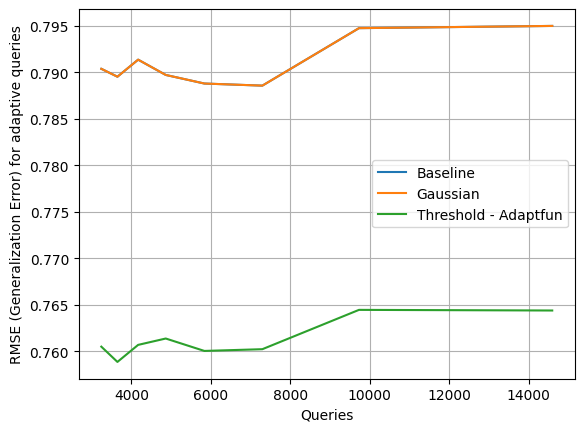
\includegraphics[width=1.0\textwidth]{c_adaptivity.png}
\caption{}
\end{centering}
\end{subfigure}
\begin{subfigure}{.32\textwidth}
\begin{centering}
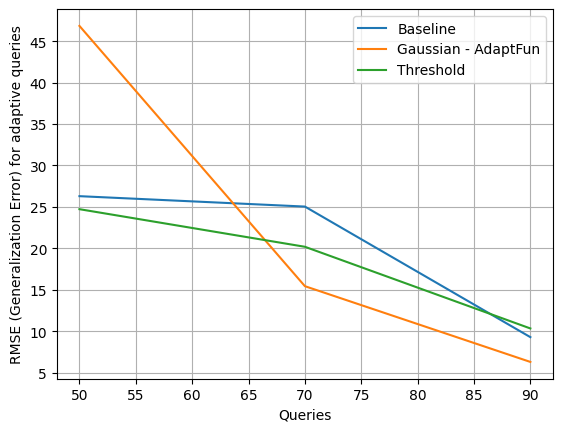
\includegraphics[width=1.0\textwidth]{n_adaptivity.png}
\caption{}
\end{centering}
\end{subfigure}
\quad
\begin{subfigure}{.3\textwidth}
\begin{centering}
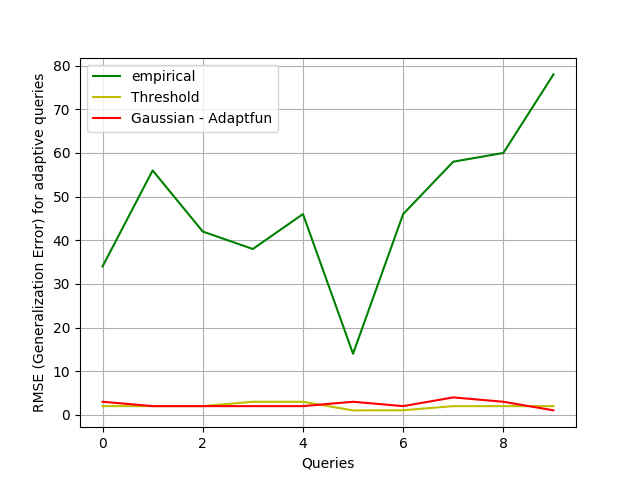
\includegraphics[width=1.0\textwidth]{exp_adaptivity.png}
\caption{}
\end{centering}
\end{subfigure}
\vspace{-0.2cm}
 \caption{The adaptive data analysis programs with
 (a) $O(1)$ adaptivity, 
 (b) $O(n)$ adaptivity,
 (c) and $O(2^n)$ adaptivity.
}
\label{fig:implementation_generalization_errors}
\vspace{-0.6cm}
\end{figure}
}
